\section{Results}
\subsection{Processing of a Single Long-Range Dependency in the Italian NLM}
We first tested whether the Italian NLM has developed a long-range agreement mechanism similar to that identified in English \citep{lakretz2019emergence}. For this, we followed the same steps described in the previous section - an ablation study, visualization of unit dynamics and a connectivity analysis. 

\subsubsection{Ablation Results} to identify unit(s) that encode grammatical number for long-range dependencies, we conducted an ablation study, as described above, using an Italian noun-PP NA-task. We found that one unit, unit 815, brings the performance of the network to around chance level in both incongruent conditions (SP and PS), i.e., whether the main subject was singular or plural (figure S1). This suggests that unit 815 encodes both singular and plural number for long-range dependencies. Note the difference with the English NLM (section \ref{}), in which two separate long-range number units have emerged. 

\subsubsection{Dynamics of the Number Unit} to further confirm that unit 815 is a long-range number unit, we visualized the dynamics of the unit during the processing of the long-range dependency, by extracting its activations during the processing of all sentences in the noun-PP NA-task. Figure \ref{fig:nounpp} describes the resulting average cell-state activations. It shows that number information is robustly encoded throughout the subject-verb dependency, across the intervening noun (attractor) - in the incongruent conditions (dashed lines), cell activity persists across the intervening noun. Consistently with the ablation results, unit 815 encodes both singular (red) and plural (blue) number, using negative and positive cell activations, respectively.

\subsubsection{Long-Range Gender Units}

\vspace{10pt}

Taken together, we replicate the main results found in the English NLM - sparse long-range number units emerge in the NLM during training. 

\begin{figure}
    \centering
    \includegraphics[width=\textwidth]{figures/model_activations_nounpp.png}
    \caption{\textbf{Cell activity of the number unit (panel A) and gender unit (panel B) during the processing of a single long-range dependency across a prepositional phrase:} four conditions are presented, corresponding to whether the main subject of the sentence is singular (red curves) or plural (blue), and to whether the main subject (`bambino') and the intervening noun (`contadino') have the same (congruent) or opposite number (incongruent)}
    \label{fig:nounpp}
\end{figure} 
\subsection{Processing of Two Long-Range Dependencies in the Italian NLM}

\subsubsection{Number-Unit Dynamics}
We next simulated NLM dynamics for all NA-tasks and conditions, by presenting all sentences from each condition to the NLM and then extracting the corresponding unit activations (methods \ref{}). Figure \ref{fig:2by2_dynamics} presents hidden-state dynamics \YL{replace with cell activation, as in figure 1} of unit 815 during the processing of all conditions of all four NA-tasks. We highlight several characteristic of the resulting dynamics: first, consistent with results on a single dependency, the grammatical number of the main subject is encoded with the same polarity - positive for plural (blue) and negative for singular (red). Second, in successive NA-tasks, the activation of unit 815 returns to baseline after encountering the main verb ('dice'), and then rises back once the main subject is encountered. This is in accordance with that unit 815 can sequentially encode the two grammatical numbers of successive dependencies. In particular, note that in the Long-Successive, the grammatical number of the embedded subject is robustly carried across the attractor 'fratello' in the incongruent conditions (blue and red dashed lines). Third, in both Short- and Long-Nested, the grammatical number of the main subject is robustly carried across the main dependency up to the main verb ('evita') \YL{fix xticklabels}, beyond the embedded subject and verb. In particular, the occurrence of opposite grammatical numbers in incongruent conditions (dashed lines) does not significantly disturb its dynamics. 

\begin{figure*}
    \centering
    \includegraphics[width=\textwidth]{figures/model_activations.png}
    \caption{\textbf{Dynamics of the hidden activation of the number unit during the processing of two subject-verb dependencies.} Number-unit activity is presented for the four structures in the design: SC-short (panel A), SC-long (B), objRC-short (C) and objRC-long (D). For each structure, results are presented for the four conditions, corresponding to whether the main subject of the sentence is singular (red curves) or plural (blue), and to whether the main and embedded subjects have the same grammatical number (congruent; continuous lines) or not (incongruent; dashed lines).}
    \label{fig:2by2_dynamics}
\end{figure*}


\subsubsection{Performance on Successive Dependencies}
Since no significant processing difficulty is predicted in the successive tasks, we focused our experiments on the embedded agreement, which is expected to be the more difficult one. This has allowed us to reduce experimental duration with human participants. Figure \ref{fig:SC_results}A presents error-rates of the NLM. To facilitate the interpretation of the results, given the relatively large number of conditions, we show the results grouped by whether the main and embedded subjects are congruent (blue) or not (red) - figure S2 provides the full error-rate distribution across all conditions. Overall, for both Short- and Long-Successive, the performance of the NLM was found to be near perfect (\YL{add stats}), with slightly more errors in the Long-Successive case (\YL{add stats}). This is consistent with the sequential encoding observed in the dynamics of the number unit (figure \ref{fig:2by2_dynamics}), which shows a robust encoding of the grammatical number of the embedded subject, also in the presence of an attractor. We next tested whether incongruent-subject conditions elicited more errors compared to congruent ones - we refer to this as \textit{subject-congruence effect}. No significant subject-congruence effect was found in neither Short- nor Long-Successive \YL{stats}.

\subsubsection{Performance on Nested Dependencies}
Figure \ref{fig:objRC_results}A presents the corresponding error-rates in the case of nested dependencies (see figure S3 for the full error-rate distribution across all conditions). Several effects are observed in the results: first, a significant subject-congruence effect was found on both the embedded and main verb, in both Short- and Long-Nested tasks (\YL{stats}). In all these cases, incongruent subjects elicited more errors compared to congruent subjects. Furthermore, a significant interaction was found between subject-congruence and verb-position in both Short- and Long-Nested tasks - increase in error-rate for incongruent-subjects was greater on the embedded compared to the main verb (\YL{stats}). Finally, a significant three-way interaction was found among subject-congruence, verb position and NA-task (Short- vs. Long-Nested), with increased error-rate in the Long-Nested task. 

\vspace{10pt}

\subsubsection{Discussion of NLM results}
The error-rate patterns of the NLM are therefore consistent with the predictions summarized in table \ref{tbl:predictions}: first, successive dependencies are relatively easy for the model, and can be processed sequentially as was confirmed by cell dynamics of the number unit (figure \ref{fig:2by2_dynamics}). Second, the main dependency in both Short- and Long-Nested was successfully processed, although with more overall errors compared to verbs in successive dependencies. Third, the NLM made an exceptionally large number of errors on the embedded verb in Long-Nested, as predicted by the sparsity of the long-range mechanism. This is apparent in incongruent-subject conditions only, in which the grammatical number of the main subject encoded in the long-range mechanism can interfere. Finally, the NLM made a relatively large number of errors on the embedded verb in Short-Nested, although still significantly above chance level ($error-rate = 0.5$; \YL{stats}). The reduced number of errors in this case, compared to that on the embedded verb in Long-Nested, is consistent with the prediction that a short-range mechanism can process the embedded dependency and compensate for the unavailability of the long-range mechanism. \YL{refer to a section in the SM, in which the effect of the attractor is analyzed}.

\subsection{Processing of Two Long-Range Dependencies in Humans}
The previous section has shown that the NLM cannot robustly encode two long-range dependencies that are active at once. The NLM was found to: (1) make an increased error rate on the embedded verb in both Short- and Long-Nested, and (2) to make an exceptionally high error-rate when the embedded dependency was long- compared to short-range. 

We next consider the number-agreement mechanism in NLMs as an informative model for agreement processing also in humans, and make the following predictions about human performance:

\begin{itemize}
    \item \textbf{Prediction 1}: humans will tend to make more agreement errors on the embedded compared to the main dependency in nested constructions. 
    \item \textbf{Prediction 2}: error-rates on the embedded verb will increase when the embedded dependency is long- compared to short-range.
\end{itemize}

We tested these predictions by presenting Italian speakers with sentences from the same four tasks in the experimental design (figure \ref{fig:design}; Methods). We then evaluated the resulting error-rates and compared them to that of the NLM, as described next. 

\subsubsection{Performance on Successive Dependencies}
Figure \ref{fig:SC_results}B presents the resulting error-rates for the successive NA-tasks. Overall, humans tend to make relatively few errors on these constructions, although significantly above zero (\YL{stats}). Note that in comparison to the Italian NLM, humans have a higher error baseline, to which unrelated factors may contribute, such as occasional lapses of attention, which are specific to humans. We found no significant subject-congruence effect in Short-Successive, and a marginally significant subject-congruence effect in Long-Successive (\YL{stats}) \YL{compare to performance on noun-PP}.

\subsubsection{Performance on Nested Dependencies}
Figure \ref{fig:objRC_results}B presents errors-rate data for the Short- and Long-Nested tasks. We highlight several effects: first, a significant subject-congruence effect was found at the embedded verb for both Short- and Long-Nested tasks (\YL{stats}). In contrast, none of the subject-congruence effects was found significant at the main verb, in neither Short- nor Long-Nested. A significant interaction was found between subject congruence and verb position, in both tasks. Finally, the three-way interaction among subject-congruence, verb position and NA-task was not found significant. However, this interaction was found significant when the main subject is plural (figure S4). 

\subsubsection{Discussion of human results}
We discuss the agreement-error patterns in humans in light of the long-range agreement mechanism. First, successive dependencies are relatively easy for humans compared to nested, without, or with only a marginal, subject-congruence effect. This is consistent with sequential processing of grammatical number by such a mechanism. Second, the main dependency in both Short- and Long-Nested was processed more robustly than the embedded one, as suggested by a significant interaction between subject-congruence and verb position, in accordance with \textit{Prediction 1} above. Finally, we found that when the main subject was plural, humans tended to make more errors when the embedded dependency was long- compared to short-range, as suggested by a significant three-way interaction among subject-congruence, verb position and task. This is in accordance with \textit{Prediction 2}. \YL{discuss markedness}


\subsection{Humans-NLM comparison}
We conclude by summarizing in table \ref{tbl:comparison} the main points of similarities and differences in agreement-error patterns between humans and NLM.

\begin{table}[h]
\tiny
\centering
\parbox{.4\linewidth}{
\centering
    \begin{tabular}{ |P{3cm}|P{1.3cm}|P{1.3cm}|  }
    \hline
    \rowcolor{cyan}
    \multicolumn{3}{|c|}{\textbf{Short-Successive}} \\
    \hline
    \rowcolor{cyan}
    \textbf{Effect} & \textbf{Humans} & \textbf{RNNs} \\
    \Xhline{3\arrayrulewidth}
    \rowcolor{green}
    \textbf{Subject Congruence (Embedded verb)} & X & X \\
    \hline
    
    \end{tabular}
}
\hfill
\parbox{.4\linewidth}{
\centering
    \begin{tabular}{ |P{3cm}|P{1.3cm}|P{1.3cm}|  }
    \hline
    \rowcolor{cyan}
    \multicolumn{3}{|c|}{\textbf{Long-Successive}} \\
    \hline
    \rowcolor{cyan}
    \textbf{Effect} & \textbf{Humans} & \textbf{RNNs} \\
    \Xhline{3\arrayrulewidth}
    \rowcolor{green}
    \textbf{Subject Congruence (Embedded verb)} & X & X \\
    \hline
    
    \end{tabular}
}

\vspace{25pt}

\parbox{.4\linewidth}{
\centering
    \begin{tabular}{ |P{3cm}|P{1.3cm}|P{1.3cm}|  }
    \hline
    \rowcolor{cyan}
    \multicolumn{3}{|c|}{\textbf{Short-Nested}} \\
    \hline
    \rowcolor{cyan}
    \textbf{Effect} & \textbf{Humans} & \textbf{RNNs} \\
    \Xhline{3\arrayrulewidth}
    \rowcolor{magenta}
    \textbf{Subject Congruence (Main verb)} & X &  V\\
    \Xhline{3\arrayrulewidth}
    \rowcolor{green}
    \textbf{Subject Congruence (Embedded verb)} & V &  V\\
    \hline
    \rowcolor{green}
    \textbf{Interaction: Subject-Congruence Verb-Position} & V &  V\\
    \hline
    
    \end{tabular}
}
\hfill
\parbox{.4\linewidth}{
\centering
    \begin{tabular}{ |P{3cm}|P{1.3cm}|P{1.3cm}|  }
    \hline
    \rowcolor{cyan}
    \multicolumn{3}{|c|}{\textbf{Long-Nested}} \\
    \hline
    \rowcolor{cyan}
    \textbf{Effect} & \textbf{Humans} & \textbf{RNNs} \\
    \Xhline{3\arrayrulewidth}
    \rowcolor{magenta}
    \textbf{Subject Congruence (Main verb)} & X &  V\\
    \Xhline{3\arrayrulewidth}
    \rowcolor{green}
    \textbf{Subject Congruence (Embedded verb)} & V &  V\\
    \hline
    \rowcolor{green}
    \textbf{Interaction: Subject-Congruence Verb-Position} & V &  V\\
    \hline
    
    \end{tabular}
}
\caption{A summary of all effects  humans and RNNs.}
\label{tbl:comparison}
\end{table}


% \subsubsection{Similarities}
% \begin{itemize}
%     \item \textbf{No significant processing difficulties on successive dependencies}: overall error-rates are relatively small, without, or with only a marginal, significant subject-congruence effect. 
%     \item \textbf{Processing difficulty on the embedded verb of a nested dependency}: More errors are observed in incongruent compared to congruent conditions on the embedded, relative to the main verb. 
%     \item {The embedded verb of a long-range nested dependency}: 
% \end{itemize}
% \subsubsection{Differences}
% \begin{itemize}
%     \item Subject-congruence effect on the main subject in NLMs but not humans. 
% \end{itemize}


\begin{figure*}[h]
    \centering
    \includegraphics[width=10cm]{figures/error_rates_successive.png}
    \caption{\textbf{Error rates on the SC-short and SC-long structures:} collected from NLMs (panel A) and human subjects (B). Blue and red bars correspond to whether the main and embedded subjects agree on number (congruent subjects) or not (incongruent), respectively). Error bars represent standard error of the mean across all trials. ns - non significant.}
    \label{fig:SC_results}
\end{figure*}


\begin{figure*}[h]
    \centering
    \includegraphics[width=10cm]{figures/error_rates_nested.png}
    \caption{\textbf{Error rates on the objRC-short and objRC-long structures:} collected from NLMs (panel A) and humans subjects (panel B). Blue and red bars correspond to whether the main and embedded subjects agree on number (congruent subjects) or not (incongruent), respectively. Error bars represent standard error of the mean across all trials. ns - non significant.}
    \label{fig:objRC_results}
\end{figure*}


% \YL{discuss marked case and the corresponding results.}

